\chapter{The System Dependence Graph} \label{ch:sdg}

As mentioned before, a system dependence graph (SDG) is a way to represent a program in its entirety as far as control 
and data dependencies are concerned. Note however that the control flow itself is not encoded in the SDG. Consider, for 
example, two statements in a procedure, which are control dependent on that procedure (meaning they will be executed 
whenever the procedure is executed). The SDG does not contain any information about the order in which those two 
statements will be executed when the procedure is called, this information is only available in the control flow graph.

The CSDG used here, in addition to control and data dependencies, also encodes variability in the form of conditions on 
edges. Those so-called presence conditions are Boolean expressions that encode for which combinations of enabled 
features an edge is present in the graph. A feature in this context is, for example, a configuration option that's read 
from a global variable. Since these conditions are of no concern to the visualization and exploration of the SDG 
itself, I will ignore them most of the time. They may however be useful in future additions to the \SB.

The following two sections will describe the implementation and construction of the SDG, and give a detailed 
explanation of its structural properties.


\section{Construction and Implementation}

The construction of the SDG is covered in great detail in Andreas Grimmer's master thesis~\cite{GrimmerDA}, the 
following section will only give a brief overview. \autoref{fig:toolchain} shows an overview of the analysis toolchain.

\begin{figure}[ht]
  \centering
    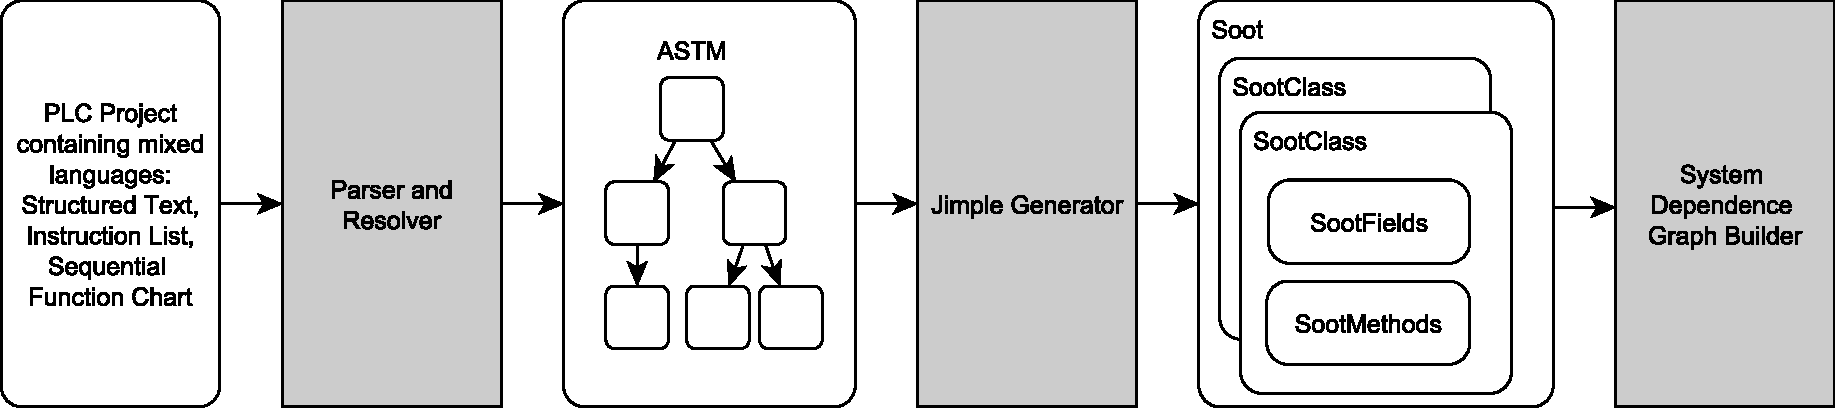
\includegraphics[width=\textwidth]{bilder/toolchain}
  \caption{Overview of the analysis toolchain for building the SDG (taken from \cite{GrimmerDA})}
  \label{fig:toolchain}
\end{figure}

The input for the SDG construction is a PLC program written in the IEC 61131-3 family of 
languages~\cite{IEC61131:2003}, specifically, a proprietary dialect of the language used by KEBA. The program is first 
parsed into an abstract syntax tree (AST) which is based on the OMG ASTM~\cite{ASTM} and was extended to handle 
features specific to the IEC languages~\cite[ch.~4]{GrimmerDA}. 

The ASTM representation serves as an input to generate Jimple code, an intermediate language representation used by the 
Soot analysis framework~\cite{Soot}. Soot is used to perform control flow and points-to analyses, and it provides 
def-use information and post-dominator trees used in the construction of the SDG.

The SDG is then created in two steps~\cite[ch.~6]{GrimmerDA}.

\begin{enumerate}
  \item In the first step, a program dependence graph (PDG) is built for each procedure in the program. The nodes in 
  this graph represent statements and formal parameters, the edges represent the intra-procedural control and data 
  dependencies. The PDGs are object-insensitive, which means they are computed once for each procedure rather than 
  based on object instances.
  
  \item The object-sensitive SDG is created by instantiating each PDG according to the object instances 
  it is used in. Information about object instances is provided by Soot's points-to analysis. The PDGs are linked by 
  introducing control edges that link calls to called procedures, and data edges between actual and formal parameter 
  nodes. Since a PLC program may have several entry points, an artificial procedure node is created for the 
  \lstinline|main| procedure, which links to every possible entry point into the program.
\end{enumerate}

\subsection{SDG Classes} \label{sec:classes}

The SDG is represented by classes \lstinline|DGNode| and \lstinline|DGEdge|, which are the abstract base classes for 
different kinds of nodes and edges, and by class \lstinline|SystemDependenceGraph|, which has the main entry point. 
\autoref{fig:classes-sdg} shows a class diagram of all SDG classes.

\begin{itemize}
  \item Each node has a list of successors and predecessors, edges which link to and from other nodes, respectively.
  
  \item A node may have a seed condition associated with it, a Boolean expression that specifies for what feature 
  combinations dependent nodes are reachable.
  
  \item A \lstinline|PDGNode| represents a statement in the program, whether it be conditional or not (to determine 
  that, information from the AST is necessary).
  
  \item There are three subclasses of \lstinline|SDGNode|, which represent procedure instances and their interactions. 
  Each \lstinline|SDGNode| has an owning \lstinline|Procedure| associated with it, which represents an instance of a 
  procedure much like a \lstinline|ProcedureNode|.
  \begin{itemize}
    \item A \lstinline|ProcedureNode| represents an instance of a procedure and may have zero or more formal parameter 
    nodes associated with it.
    
    \item \lstinline|ExprNode| may represent formal or actual parameters, as well as global variables. In the case of a 
    formal parameter node for a global variable accessed by the procedure, the node also refers to the actual node 
    representing the global variable itself.
    
    \item Calls between procedures are represented by \lstinline|ActivationNode|s. An activation node refers to the 
    statement that represents the call, has one or more procedures that are called (more than one procedure may be 
    called, e.g.\ by setting an event, which may trigger several event handlers), and has all actual parameters for the 
    call attached to it.
  \end{itemize}
  
  \item An edge may have a presence condition associated with it, a Boolean expression that specifies for what feature 
  combinations the edge does exist.
  
  \item A \lstinline|ControlEdge| has an associated label, which in the case of conditional statements specifies 
  whether the control dependency is for the \lstinline|true| or \lstinline|false| branch of the condition.
\end{itemize}

\begin{figure}[hpb]
  \centering
    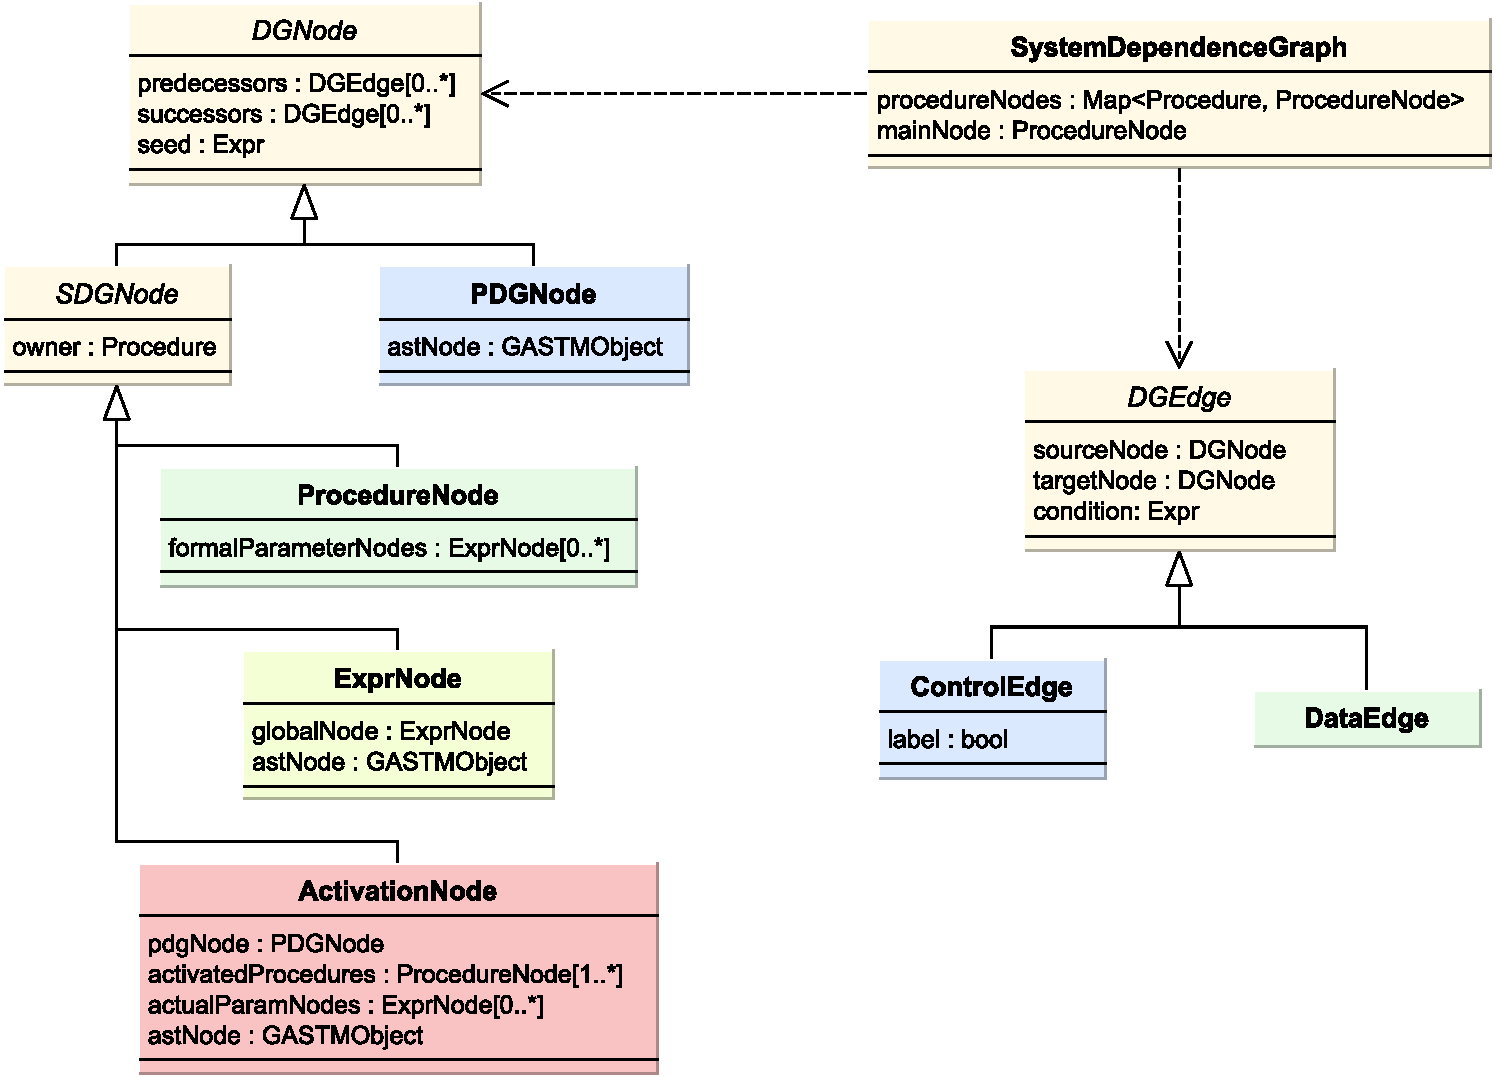
\includegraphics[width=\textwidth]{bilder/classes-sdg}
  \caption{Class diagram of the SDG classes}
  \label{fig:classes-sdg}
\end{figure}


\section{Structure}

This section will explain the structure of the underlying SDG in detail, and also the changes and simplifications made 
for display to the user. Because not everything one might want to explore is represented in the SDG (for example, local 
variables don't have a representation in the SDG) additions are also mentioned.

% Alternative 1: several gradually bigger examples

\subsection{Overview}

The rough structure of the SDG is best explained by means of an example: the program in \autoref{lst:csdg-simple} uses 
two load-time configuration options and contains conditional statements and method calls. The CSDG corresponding to the 
program can be seen in \autoref{fig:csdg-simple}; note that this SDG is greatly simplified, but will suffice for a 
rough overview.

The procedure nodes in green correspond to the two methods in the program, \lstinline|main| and \lstinline|foo|. 
Control edges in blue and red (for the \lstinline|true| and \lstinline|false| branch of a conditional, respectively) 
connect control dependent statements to procedures and conditional statements. Note that conditional statements are 
represented by statement nodes just like ordinary statements. The SDG itself does not contain any information about 
whether a statement is a condition or not, this information is taken from the AST nodes linked to each statement node. 
Dashed edges show the flow of data between different nodes, from the writing to the reading node.

In the CSDG, edges are annotated with their respective presence conditions, which depend on the two configuration 
options. Seed conditions (not shown in the figure), as mentioned in \autoref{sec:classes}, are present on the three 
conditional nodes and serve as the initial conditions for the propagation of presence conditions. A detailed 
explanation of the process of finding configuration options and augmenting the SDG with presence conditions can be 
found in \cite{DBLP:conf/kbse/AngererGPG15}. Note that in this example only some of the presence conditions are shown.

This can also serve as an example of using the CSDG for configuration-aware change impact analysis: say we want to know 
whether a change to the highlighted return statement in method \lstinline|foo| would affect the print statement. Then 
we can see that the conditions of the data edge from the return to the print statement ($ \lnot c_1 \land c_0 $) and 
the print statement's incoming control edge ($ \lnot c_0 $) are disjoint, they cannot both be true
(i.e.\ $ \left( \lnot c_1 \land c_0 \right) \land \lnot c_0 \implies \text{False} $). This means that a change to the 
return statement does not affect the print statement, while we would have concluded that it does, had we ignored 
variability information provided by the configuration options.

\begin{lstlisting}[float=p,label=lst:csdg-simple,
  caption={Program using load-time variability resulting in the SDG in \autoref{fig:csdg-simple}}]
class Main {
  final boolean c0 = getConfiguration("c0");
  final boolean c1 = getConfiguration("c1");
  
  public void main(String[] args) {
    int res = 0;
    if(c0) {
      res = foo();
      return;
    } else if(c1)
      res = foo();
    System.out.println(res);
  }
  
  private int foo() {
    if(!c1)
      (@@)`return 1`;
    return 0;
  }
}
\end{lstlisting}

\begin{figure}[p]
  \centering
    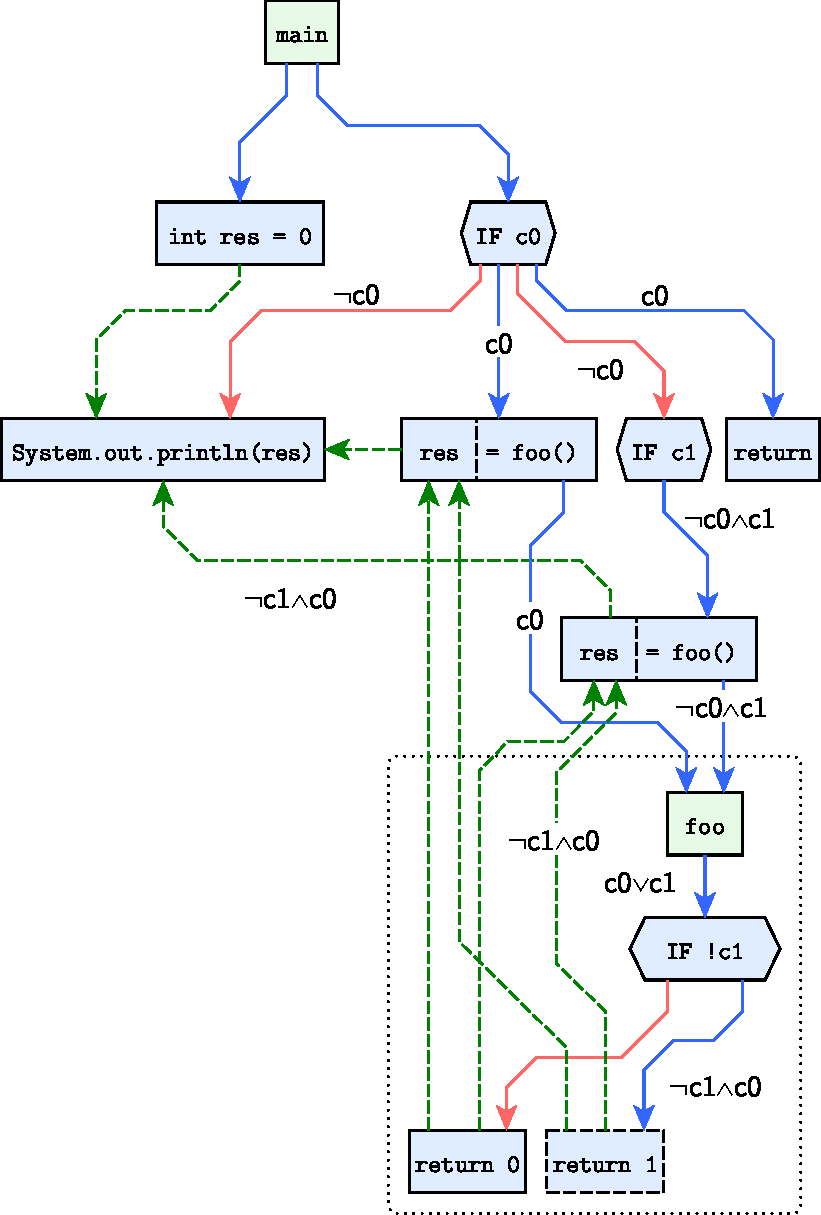
\includegraphics[scale=0.6]{sdgs/simple-csdg}
  \caption{Simplified CSDG for the sample program in \autoref{lst:csdg-simple}}
  \label{fig:csdg-simple}
\end{figure}


\subsection{Calls}

Let's first look at an example of function calls: the program in \autoref{lst:sdg-calls} calls two methods with one 
parameter each, one of the methods uses a global variable as well. \autoref{fig:sdg-calls} show the corresponding SDG. 
The SDG now contains two additional node types: activation nodes (call nodes) are shown in red, while three different 
kinds of expression nodes are shown in orange.

Global variables are represented in the SDG by expression nodes attached to the main procedure node via control edges. 
These are semantically variable nodes.

The parameters to procedures are represented by expression nodes (semantically those are formal parameter nodes) 
attached to their procedure node via control edges (which semantically are parameter edges, shown dotdashed in the 
figure). The procedure \lstinline|foo| has an additional formal parameter node that represents the global variable, 
since that can be seen as a hidden parameter.

A call is represented by an activation node, the parameters to the call are also represented by expression nodes (which 
semantically are now actual parameter nodes), attached again via parameter edges. The statement causing a call links to 
the activation node via a control edge, the activation node in turn is also linked to the activated procedures (which 
may be more than one) via control edges (which can be seen semantically as call edges). Note however that one statement 
calling more than one procedure (e.g.\ \lstinline|bar(foo(42));|) is still represented by multiple activation nodes in 
the SDG; a single activation node for multiple activated procedures happens only in case of, for example, IEC events, 
where one expression may cause a number of event handlers to be executed. If a procedure returns one or more values 
(more than one value may be returned via output parameters in IEC procedures), these will be represented by formal 
parameter nodes as well.

Generally the \SB will not make a visual distinction between different kinds of control edges or parameter nodes, only 
variable nodes will be distinguished from other expression nodes for clarity.

Data flow, instead of going directly in and out of a procedure's PDG, now takes an indirection over the procedure's 
formal parameter nodes. Generally there will be data edges connecting some nodes to an actual parameter node, which in 
turn connects to the formal parameter node, which then connects to statements inside the procedure. Data flow out of 
the procedure works much the same, with data edges connecting statements to formal parameter nodes for output 
parameters. Note that in the IEC language there are also in-out parameters, which may have data flowing in both 
directions. Similarly, reading from and writing to global variables takes an indirection over the corresponding formal 
parameter node.

\begin{lstlisting}[float=p,label=lst:sdg-calls,
  caption={Program with calls resulting in the SDG in \autoref{fig:sdg-calls}}]
class Main {
  static int global = 1;
  
  public static void main(String[] args) {
    boolean res1 = foo(42);
    int res2 = bar(res1);
    System.out.println(res2);
  }
  
  private static boolean foo(int n) {
    if(n < global)
      return false;
    gloabl = n;
    return true;
  }
  
  private static int bar(boolean b) {
    if(b)
      return 2;
    return 3;
  }
}
\end{lstlisting}

\begin{figure}[p]
  \centering
    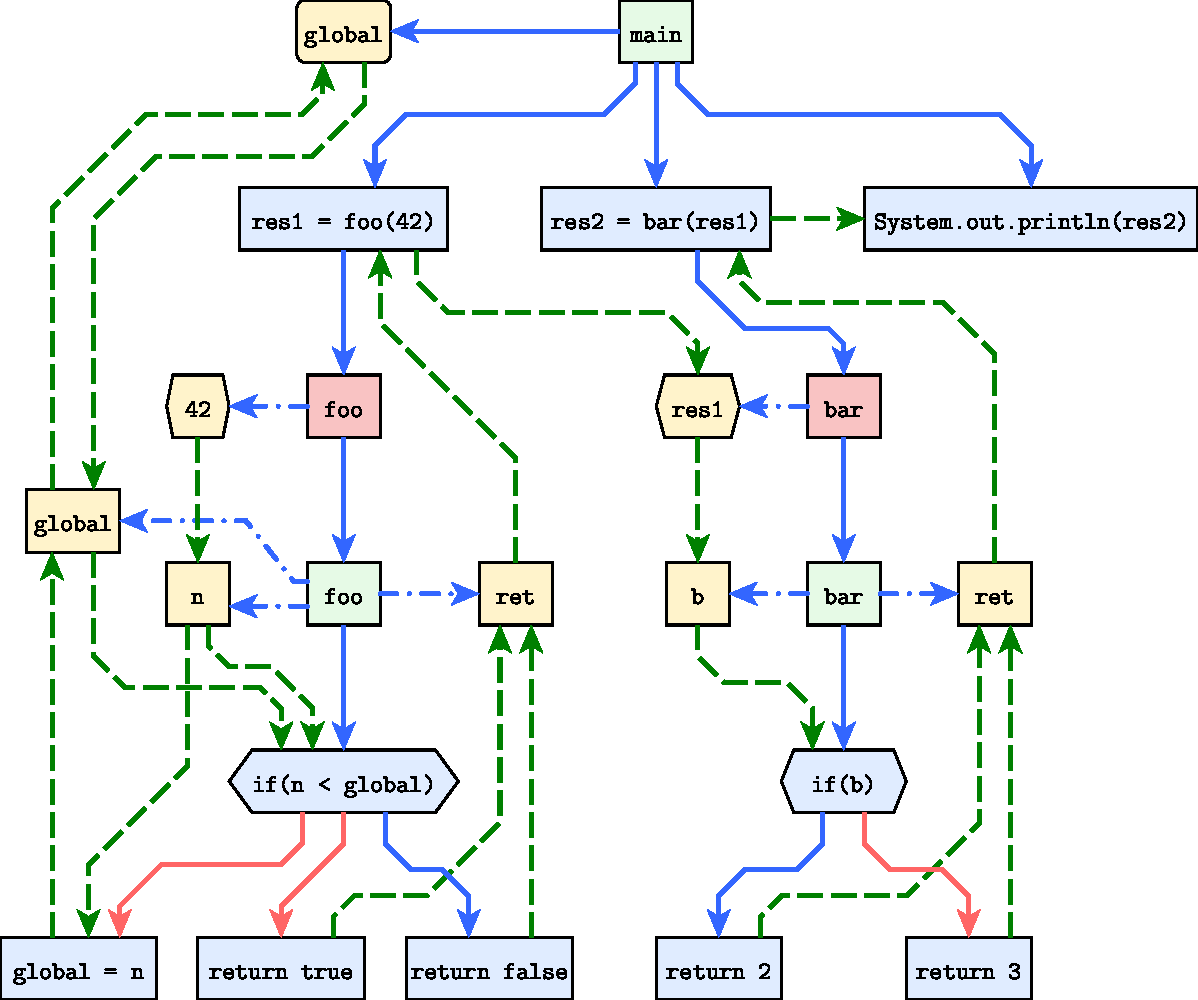
\includegraphics[scale=0.6]{sdgs/calls}
  \caption{SDG for the sample program in \autoref{lst:sdg-calls}}
  \label{fig:sdg-calls}
\end{figure}

